\section{Methods}

\subsection{Design requirements}

The jaw makes essential contributions to the chewing process such as generating the forces required to break down food, controlling the lower mandible motion
and giving sensory feedback. A robotic jaw should therefore be able to mimic these functions as closely as possible.
As this is the first iteration of the chewing robot, we focus on force generation and range of motion, while sensory feedback and other functions can be added in future iterations.
The design requirements are based on the literature and the human jaw anatomy and physiology, as summarized in Table~\ref{tab:functional_criteria}.
Note that the jaw's speed is not a design requirement as food can be effictively chewed even at slow speeds.

\begin{table}[H]
  \centering
  \begin{tabular}{@{}L{4.2cm}L{6.4cm}L{4.2cm}@{}}
    \toprule
    \textbf{Quantity} & \textbf{Values reported in the literature} & \textbf{Design requirement} \\
    \midrule
    Degrees of freedom (DoF) 
      & 6 DoF: 3 translational (X, Y, Z) and 3 rotational (roll, pitch, yaw) \cite{6dof}
      & 6 DoF \\[2pt]
    \hline
    Vertical (compressive) bite force $F_{z}$ 
      & $600$ N chewing force in healthy adults \cite{chewing_force},\; $1243$ N maximum clenching force \cite{max_clenching_force}
      & $800$ N \\[2pt]
    
    \hline

    Lateral force $F_{x}$ 
      & $-72$ N (left) to $+53$ N (right) during maximal biting \cite{shear_force}
      & $\pm100$ N \\[2pt]
    \hline

    Anterior–posterior force $F_{y}$ 
      & $-10$ N (posterior) to $+30$ N (anterior) \cite{shear_force}
      & $\pm50$ N \\[2pt]
    \hline

    Mandibular motion range 
      & $14$ mm lateral shift, $11$ mm protrusion, $61$ mm mouth opening in healthy adults \cite{range_motion_required}
      & $\pm20$ mm (X, Y);\;\; $0$–$60$ mm (Z) \\[2pt]
  \bottomrule
  \end{tabular}
  \caption{Functional design requirements.}
  \label{tab:functional_criteria}
\end{table}


\subsection{Mechanical design}
\begin{itemize}
    \item goal is to create a robotic jaw that can mimic the motion and force of human chewing 
    \item 6dof stewart platform to be able to mimic the motion of the jaw
    \item linear actuators instead of rotary servo motors to have more efficient force transmission + simpler kinematics + more rigid structure
    \item choice of actuators based on the required force to mimic human chewing (speed less important as jaw can chew even if slow) + required length to 
    reach the desired range of motion + feedback to control in position
    \item choosing the dimensions of the stewart platform based on the size of the actuators + working space of the robot
    \item choice of structure/material to hold upper jaw to be rigid enough to not deform under the forces applied by the actuators 
    \item 3 axis load cells to measure the force applied by the jaw
    \item so far 3d printed teeth/jaw but to be changed in the future
\end{itemize}


\subsection{Control}

%The control layer combines a high-speed microcontroller, a modular C++ codebase, and classical PI loops to deliver real-time motion of 
%the Stewart platform.  Figure~\ref{fig:code_structure} gives the software context, while the full electronics schematic is shown in 
%Fig.~\ref{fig:elec_schematic}.

\subsubsection{Hardware (electronics)}
A Teensy~4.1 (600 MHz ARM Cortex-M7, single-precision FPU) executes the control loop.% at \SI{100}{\hertz}. %? %todo: add ref for the freq/reason
Its key peripherals are:  
\begin{itemize}[nosep]
    \item three \SI{12}{\ampere} dual DC motor drivers (DF Robot) controlling the six linear actuators;
    \item six analogue inputs reading potentiometer position feedback from the linear actuators;
    \item three transmitters for the load cells mounted on top of the maxilla;
    \item an on-board micro-SD slot used for trajectory files and calibration data.
\end{itemize}
A \SI{12}{\volt} AC/DC brick powers the actuators directly; the user's computer supplies \SI{5}{\volt} to the Teensy, which in 
turn sources the \SI{3.3}{\volt} logic rails for the motor drivers and load-cell transmitters.
The full electronics schematic is shown in Fig.~\ref{fig:elec_schematic}.

\begin{figure}[H]
\centering
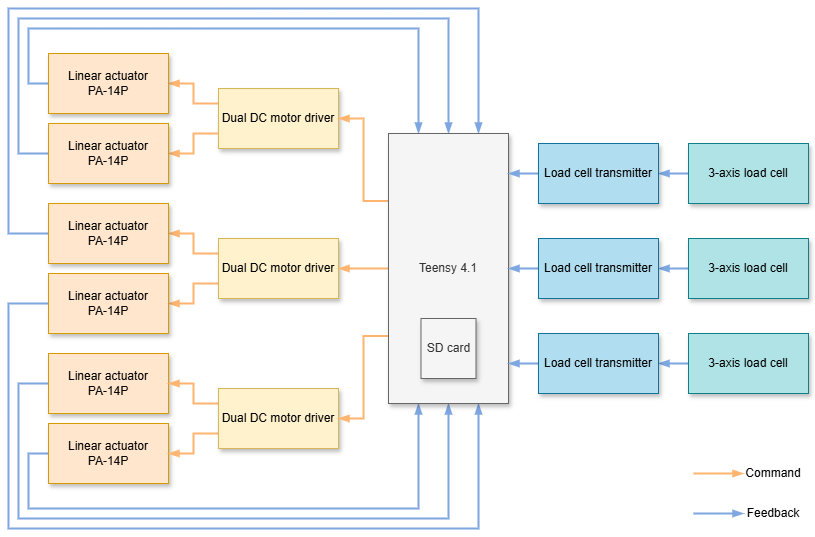
\includegraphics[width=\textwidth]{figures/elec_schematic.drawio.png}
\caption{Electronics schematic.}
\label{fig:elec_schematic}
\end{figure}

\subsubsection{Software architecture}
The central class \texttt{RobotController} maintains the finite-state machine in Fig.~\ref{fig:state_machine} and manages two
 modules:  
\begin{itemize}[nosep]
    \item \texttt{StewartPlatform}: inverse kinematics, trajectory interpolation, and low-level actuator commands;
    \item \texttt{ForceSensing}: continuous load-cell acquisition and filtering;
\end{itemize}
The controller is designed to be modular, allowing for easy addition of new modules such as a tongue or saliva module in the future.
The three controller states are:
\begin{enumerate}
    \item \textbf{Stop} – return to home pose; reload trajectory if the user selects a new file;
    \item \textbf{Calibrate} – user can manually change the initial $(x,y,z)$ position via the GUI;
    \item \textbf{Move} – replay the selected trajectory.
\end{enumerate}
A lightweight Python GUI on the host PC issues high-level commands, such as state changes, and plots sensor data.  

    

\begin{figure}[H]
\centering
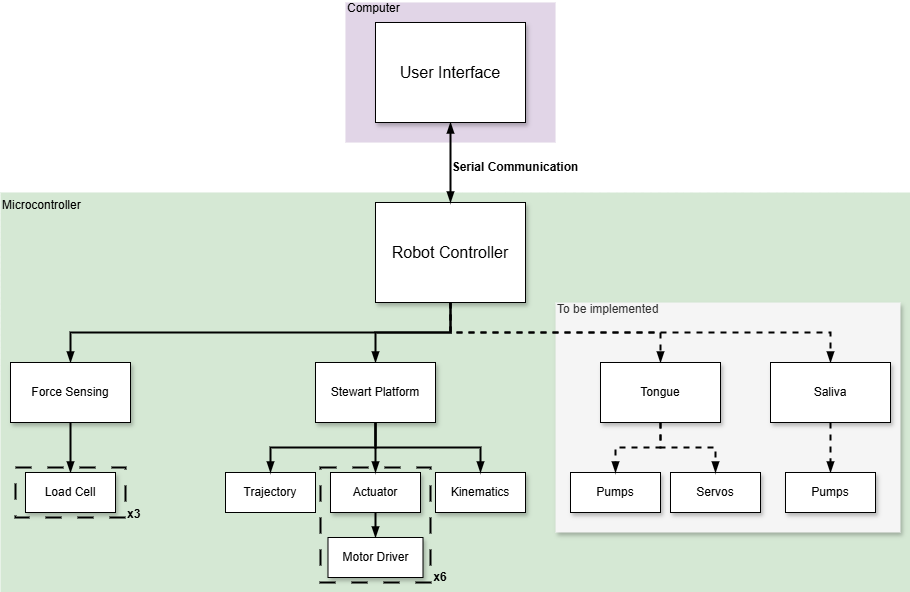
\includegraphics[width=\textwidth]{figures/code_structure.drawio.png}
\caption{Overall code structure.}
\label{fig:code_structure}
\end{figure}


\begin{figure}[H]
\centering
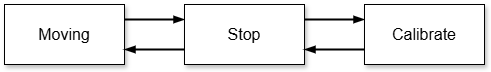
\includegraphics[width=0.6\textwidth]{figures/state_machine.drawio.png}
\caption{Robot controller state machine.}
\label{fig:state_machine}
\end{figure}

\subsubsection{Position control}

The Stewart Platform follows a 3D trajectory (x, y, z, roll, pitch, yaw) from a .csv file on the micro-SD card.
See section \ref{sec:motion-capture} for details on the recording protocol and data processing.
Each pose is defined by its position ${\bf t}=(x,y,z)$ and orientation given by the Euler angles $(\phi,\theta,\psi)$,
 which are the roll, pitch, and yaw angles respectively.
The trajectory is then linearly interpolated with a fixed time step chosen by the user.

\paragraph{Inverse kinematics}
For each pose in the trajectory, \texttt{Kinematics} computes the lengths of the six linear actuators that will achieve 
the desired pose of the platform, i.e. the inverse kinematics. To do so, we first compute the standard rotation matrix 
$R(\phi,\theta,\psi)$ for the Euler angles, which is defined as the product of three rotation matrices about 
the $Z$, $Y$, and $X$ axes:
\[
R(\phi,\theta,\psi) = R_Z(\psi) R_Y(\theta) R_X(\phi) =
\begin{pmatrix}
\cos\psi & -\sin\psi & 0 \\
\sin\psi & \cos\psi & 0 \\
0 & 0 & 1
\end{pmatrix}
\begin{pmatrix}
\cos\theta & 0 & \sin\theta \\
0 & 1 & 0 \\
-\sin\theta & 0 & \cos\theta
\end{pmatrix}
\begin{pmatrix}
1 & 0 & 0 \\
0 & \cos\phi & -\sin\phi \\
0 & \sin\phi & \cos\phi
\end{pmatrix}
\]

The platform joints ${\bf p}_i$, $i$ being the actuator index, are then rotated about a fixed point ${\bf c}$, 
which is the front of the gnathion, and translated by the user-defined home position ${\bf t}=(x,y,z)$, 
resulting in the world coordinates of the platform joints:
\[
{\bf w}_i = R\bigl({\bf p}_i-{\bf c}\bigr)+{\bf c}+{\bf t}.
\]

Finally, the actuator length is the Euclidean distance to the fixed base joint ${\bf b}_i$:
\[
\ell_i = \lVert {\bf w}_i-{\bf b}_i\rVert_2.
\]

\paragraph{PI controller}
For each actuator, its desired length is sent to a PI position controller, see Figure~\ref{fig:actuator_pi}.
To minimize the noise of the potentiometer feedback, we apply a low-pass filter averaging the last 10 samples.
\begin{figure}[H]
\centering
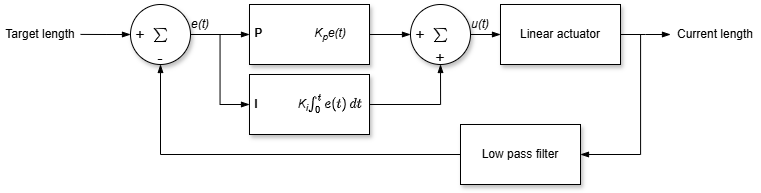
\includegraphics[width=\textwidth]{figures/actuator_pi.drawio.png}
\caption{Position PI controller for the linear actuators.}
\label{fig:actuator_pi}
\end{figure}

\subsection{Data acquisition and processing}
\label{sec:motion-capture}

\paragraph{Subjects.} 
Two healthy adult volunteers (author and project supervisor) participated in this pilot recording. Owing to time constraints and the exploratory 
nature of the study, no additional subjects were recruited.

\paragraph{Motion-capture acquisition.}
Mandibular motion was recorded with a five-camera OptiTrack system sampling at 120 Hz.
Four reflective markers arranged in a square were attached to the forehead and served as a head-fixed reference frame.
A second set of three markers forming a triangle was placed on the gnathion.
Two additional lip markers were recorded but later discarded because a single marker cannot encode orientation. \cite{motion_capture_adult,motion_capture_children}

The subject then performed the motion sequences listed in Table~\ref{tab:recording-protocol}. Each frame was saved by Motive as a \texttt{.csv} file that contains
the 3-D marker positions (in millimetres) and the orientation of each marker set as quaternions. The calibrated volume had a residual error of $0.3\,$mm.
% TODO: insert a photograph of the marker placement

\begin{table}[H]
  \centering
  \small                                   
  \renewcommand{\arraystretch}{1.1}  
  \begin{tabularx}{\textwidth}{@{} c l l @{}}      
    \toprule
    \textbf{Food} & \textbf{Motion} & \textbf{\textit{Optional:} Duration} \\
    \midrule
    % ---------- Empty mouth block ----------
    Empty mouth & 20$\times$ open–close cycles                 & —     \\[1pt]
    \midrule
    % ---------- Chewing-gum block ----------
    \multirow{5}{*}{\parbox[c]{3.2cm}{\centering Chewing gum\\(Xylit-Pro,\\\emph{Excitemint})}}
      & Random side chewing                                    & 2 min \\[1pt]
      & Right-side chewing                                     & 1 min \\[1pt]
      & Left-side chewing                                      & 1 min \\[1pt]
      & Front-teeth-only chewing                               & 1 min \\ 
    \midrule
    % ---------- Biscuit block ----------
    \multirow{5}{*}{\parbox[c]{3.2cm}{\centering Biscuits\\(Bretzeli, \emph{Kambli})}}
      & random chewing                                    & — \\[1pt]
      & front-teeth chew → right-side chew                & — \\[1pt]
      & front-teeth chew → left-side chew                  & — \\[1pt]
      & \textit{fast} random chewing                      & — \\[1pt]
      & \textit{slow} random chewing                       & — \\
    \bottomrule
  \end{tabularx}
  \caption{Recording protocol. \textit{Notes:}  
  For chewing-gum trials the first run began with an unchewed piece and the same gum was kept for all subsequent motions.  
  For biscuit trials each run started with an empty, closed mouth; the subject then placed a biscuit, chewed as instructed, and swallowed.}
  \label{tab:recording-protocol}
\end{table}

\paragraph{Data processing.}
To reduce the noise, we apply a 4th-order butterworth filter to the data. The cutoff frequency is set to 6Hz, as human mastication frequency is around 1Hz to 2Hz %\cite{chewing_frequency} TODO: find paper
. \\
The data is then transformed to the head reference frame using rotation matrices. 







